\setAuthor{Tundmatu autor}
\setRound{lahtine}
\setYear{2004}
\setNumber{G 1}
\setDifficulty{2}
\setTopic{Dünaamika}

\prob{Viplala}
Viplala tahab liigutada laua peal olevat klotsi. Selleks valmistab ta bloki abil süsteemi, et ära kasutada endale mõjuvat raskusjõudu ja nihutada klotsi, lastes ennast nööri otsa rippu (vt. joonist). Ta laskub põrandale kõrguselt $H=\SI{1}{m} .$ Oletame, et nöör ei veni, blokk on ideaalne ja klots jääb tervenisti lauale.\\
\osa Viplala valib liigutamiseks endast 2 korda raskema klotsi. Hõõrdetegur laua ja klotsi vahel on $\mu=\num{0,3}$. Kui kaua kestab Viplala laskumine laualt põrandani? Raskuskiirendus $g=\SI{10}{m/s^2}$.\\
\osa Mitu korda endast raskemat klotsi jõuaks Viplala maksimaalselt veel antud viisil nööri otsas laskudes liigutada? Eeldada, et nööri otsas sipeldes suudab ta kompenseerida suurema seisuhõõrdeteguri alghetkel, kui klots on paigal.
\begin{center}
	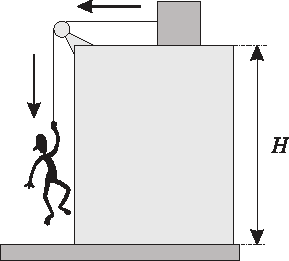
\includegraphics[width=0.4\linewidth]{2004-lahg-01-yl.pdf}
\end{center}

\hint
Kuna plokk on paigal ja nöör on venimatu, hakkavad Viplala ja klots võrdse kiiruse ja võrdse kiirendusega liikuma. Edasi tasub Viplala ja klotsi jaoks Newtoni teise seaduse kirja panna.

\solu
Olgu Viplala mass $m$, klotsi mass on seega $2 m$. Viplala tõmbab allapoole raskusjõud $m g$ ja ülesse nööri tõmbejõud $T$. Klotsi paneb liikuma nööri tõmbejõud $T$ ja takistab liikumist hõõrdejõud $2 \mu \mathrm{mg} .$ Saame kirja panna võrrandiste süsteemi:
$$
m g-T=m a, \quad T-2 \mu m g=2 m a.
$$
Lahendades võrrandisüsteemi, saame
$$
m g-2 \mu m g=3 m a \quad \Rightarrow \quad a=\frac{(1-2 \mu) g}{3}.
$$
Aja $t$ jooksul läbib Viplala tee $S=a t^{2} / 2$, seega laskumiseks kulub aeg
$$
t=\sqrt{\frac{2 S}{a}}=\sqrt{\frac{2 S \cdot 3}{(1-2 \mu) g}} \approx \SI{1,2}{s}.
$$
Viplala saab laskuda, kui kiirendus on minimaalselt null ehk toimub ühtlane liikumine. Seega
$$
m g=M \mu g \Rightarrow \frac{M}{m}=\frac{1}{\mu} \approx \num{3,3}.
$$
See tähendab, et Viplala saab liigutada klotsi, mis on temast \num{3,3} korda raskem.
\probend